\documentclass[10pt,a4paper]{article}

% Marges du document %
\setlength{\topmargin}{0cm}
\setlength{\headheight}{0.4cm}
\setlength{\headsep}{0.8cm}
\setlength{\footskip}{1cm}
\setlength{\textwidth}{17cm}
\setlength{\textheight}{25cm}
\setlength{\voffset}{-1.5cm}
\setlength{\hoffset}{-0.5cm}
\setlength{\oddsidemargin}{0cm}
\setlength{\evensidemargin}{0cm}

\usepackage{amssymb}
\usepackage{psfrag}
\usepackage[utf8]{inputenc}
\usepackage[francais]{babel}
\usepackage[T1]{fontenc}
\usepackage{amsmath}
\usepackage{amsfonts}
\usepackage{amssymb}
\usepackage{graphicx}
\usepackage{subcaption}
\usepackage{fancyhdr}
\usepackage{multicol}
\usepackage{eurosym} % symbole €
\usepackage{siunitx}
\usepackage{stmaryrd}
\usepackage{bm}

\usepackage{tabu}
\def\€{\euro{}}

\numberwithin{equation}{section}

\newcommand\numberthis{\addtocounter{equation}{1}\tag{\theequation}} 

\usepackage{color} % gestion de différentes couleurs
\definecolor{linkcolor}{rgb}{0,0,0}
\definecolor{linkcolorurl}{rgb}{0,0,1}
\usepackage[ pdftex,colorlinks=true,
pdfstartview=FitV,
linkcolor= linkcolor,
citecolor= linkcolor,
urlcolor= linkcolorurl,
hyperindex=true,
hyperfigures=false]
{hyperref} % fichiers pdf 'intelligents', avec des liens entre les références, etc.

% En-tête et pied de page % 
\pagestyle{fancy}
\fancyhead[L]{\scriptsize \textsc{Titre}} 
\fancyhead[R]{\scriptsize \textsc{BUNEL Félix et VERGNET Hadrien}} 
\fancyfoot[C]{ \thepage}

\author{Bunel Félix et Vergnet Hadrien}

%%%%%%%%%%%%%%%%%%%%%%%%%%%%%
% Tikz packages and settings
%%%%%%%%%%%%%%%%%%%%%%%%%%%%%

\usepackage{tikz}
\usepackage{pgfplots}
\usepackage{tikz-3dplot}
\pgfplotsset{compat=1.11}

\usetikzlibrary{shapes.geometric,calc,intersections}
\usetikzlibrary{shapes.arrows}
\usetikzlibrary{shadings}
\usetikzlibrary{patterns}
\usetikzlibrary{decorations.pathmorphing}
\usetikzlibrary{decorations.pathreplacing}


\usetikzlibrary{external}
\tikzset{external/aux in dpth={false}}
\tikzset{external/up to date check={simple}}
\tikzset{external/optimize command away={\includetexgraphics}{2}}

\tikzset{>=stealth}

%%%%%%%%%%%%%%%%%%%%%%%%%%%%%%%%%%%%%%%%%%%%%%%%%%%%%%%%%%%%
% Custom macro to input a tikz picture and setting its name
%%%%%%%%%%%%%%%%%%%%%%%%%%%%%%%%%%%%%%%%%%%%%%%%%%%%%%%%%%%%

\makeatletter
\newcommand{\includetikzgraphics}[1]{
	\filename@parse{#1}
	\tikzsetnextfilename{\filename@base}
	\input{#1}
}
\makeatother

%%%%%%%%%%%%%%%%%%%%%%%%%%%%%%%%%%
% Custom tikz command for drawing
%%%%%%%%%%%%%%%%%%%%%%%%%%%%%%%%%%

\tikzset{math3d/.style=
    {z= {(-0cm,-0.3cm)}, y={(0cm,1cm)},x={(1cm,0cm)}}}

% \drawYNema {x} {y} {yAngle}
\newcommand{\drawYnema}[3] {
	\shade [ball color=black] (#1,#2) ellipse 
		[x radius={sqrt(pow(cos(#3)*0.1,2)+pow(sin(#3)*0.3,2))}, y radius=0.1];
}
% \drawXNema {x} {y} {xAngle}
\newcommand{\drawXnema}[3] {
	\shade [ball color=black] (#1,#2) ellipse 
		[y radius={sqrt(pow(cos(#3)*0.1,2)+pow(sin(#3)*0.3,2))}, x radius=0.1];
}
% \drawZNema {x} {y} {zAngle}
\newcommand{\drawZnema}[3] {
	\shade [ball color=black] (#1,#2) ellipse 
		[x radius=0.3, y radius=0.1, rotate={#3}];
}

% \plotcylinder { radius } { heigth } { altitude }
\newcommand{\plotcylinder}[3] {
     \draw [math3d, fill=white, samples=100]
        plot[domain=-pi:pi] ({#1*cos(\x r)},#3,{#1*sin(\x r)}) ;
     \draw [math3d, fill=white, samples=100]
        plot[domain=0:pi] ({#1*cos(\x r)},#3,{#1*sin(\x r)}) --
        plot[domain=pi:0] ({#1*cos(\x r)},{#3-#2},{#1*sin(\x r)}) --
        cycle;
}

% \plotpolarizer { x} { y} { z } { radius } { angle }
\newcommand{\plotpolarizer}[5] {
    \draw [math3d, fill=gray, opacity=0.8, samples=100]
        plot[domain=-pi:pi] ({#1+#4*cos(\x r)},#2,{#3+#4*sin(\x r)}) ;
    \draw [math3d, opacity=0.8]
        ({#1+#4*cos(#5)},#2,{#3+#4*sin(#5)}) -- ({#1-#4*cos(#5)},#2,{#3-#4*sin(#5)}) ;
}

% \fancyarrow {xi} {yi} {xf} {yf} {width} {options}
\newcommand{\fancyarrow}[6]{
	\pgfmathsetmacro{\dx}{#3-#1};
	\pgfmathsetmacro{\dy}{#4-#2};
	\pgfmathsetmacro{\dl}{sqrt(\dx*\dx+\dy*\dy)};
	\pgfmathsetmacro{\dw}{#5/2};
	\pgfmathsetmacro{\cos}{\dx/\dl};
	\pgfmathsetmacro{\sin}{\dy/\dl};
	\draw [#6] (#1,#2) -- ++($\dw*(\sin,-\cos)$) 
		-- ++(${\dl-2*\dw}*(\cos,\sin)$)
		-- ++($\dw*(\sin,-\cos)$) -- ++($2*\dw*(\cos,\sin)+2*\dw*(-\sin,\cos)$) 
		-- ++($-2*\dw*(\cos,\sin)+2*\dw*(-\sin,\cos)$) -- ++($\dw*(\sin,-\cos)$)
		-- ++(${2*\dw-\dl}*(\cos,\sin)$) -- cycle;
}

%%%%%%%%%%%%%%%%%%%%%%%
% Custom pgf mark list
%%%%%%%%%%%%%%%%%%%%%%%
\pgfplotscreateplotcyclelist{colorhollowmarks}{%
	{black,mark=x},
	{cyan,mark=+},
	{magenta,mark=o},
	{teal,mark=square},
	{violet,mark=triangle},
	{gray,mark=diamond},
	{brown,mark=pentagon},
	{orange,mark=otimes},
	{lime,mark=10-pointed star}}
\pgfplotscreateplotcyclelist{hollowmarks}{%
	{mark=x},
	{mark=+},
	{mark=o},
	{mark=square},
	{mark=triangle},
	{mark=diamond},
	{mark=pentagona},
	{mark=otimes},
	{mark=10-pointed star}}
\pgfplotscreateplotcyclelist{onlycolors}{%
	black,
	cyan,
	magenta,
	teal,
	violet,
	lightgray,
	brown,
	orange,
	lime}



\begin{document}

%%%%%%%%%%%%%%%%%%%%%%%%%%%%%%%%%%%%%%%%%%%%%%%%%%%%%%%%%%%%%%%%%%%%%%%%%%%%%%%%%%%%%%%%
%%%%%%%%%%%%%%%%%%%%%%%%%%%%%%%%%%%%%%%%%%%%%%%%%%%%%%%%%%%%%%%%%%%%%%%%%%%%%%%%%%%%%%%%
\begin{titlepage}
%%%%%%%%%%%%%%%%%%%%%%%%%%%%%%%%%%%%%%%%%%%%%%%%%%%%%%%%%%%%%%%%%%%%%%%%%%%%%%%%%%%%%%%%
%%%%%%%%%%%%%%%%%%%%%%%%%%%%%%%%%%%%%%%%%%%%%%%%%%%%%%%%%%%%%%%%%%%%%%%%%%%%%%%%%%%%%%%%
\thispagestyle{empty}
\setlength{\parindent}{0pt}


\includegraphics[height=1.9cm]{logo-ens.jpg} \hfill 
\includegraphics[height=2cm]{logo_lyon1.jpg} \hfill 
\includegraphics[height=2cm]{logo_univ_lyon.jpg}



Master Sciences de la matière
\hfill
Projet de Géophysique

\textit{École Normale Supérieure de Lyon}
\hfill
BUNEL Félix et VERGNET Hadrien

\textit{Université Claude Bernard Lyon 1}
\hfill
M2 Physique 2015-2016
\vspace{0.5cm}

\hrulefill
\vspace{-0.6cm}

\hrulefill
\begin{center}\bfseries
\begin{huge}
    Titre
\end{huge}
\Large
\vspace{0.4cm}

Sous-titre
\end{center}
\hrulefill
\vspace{-0.6cm}

\hrulefill


\begin{center}
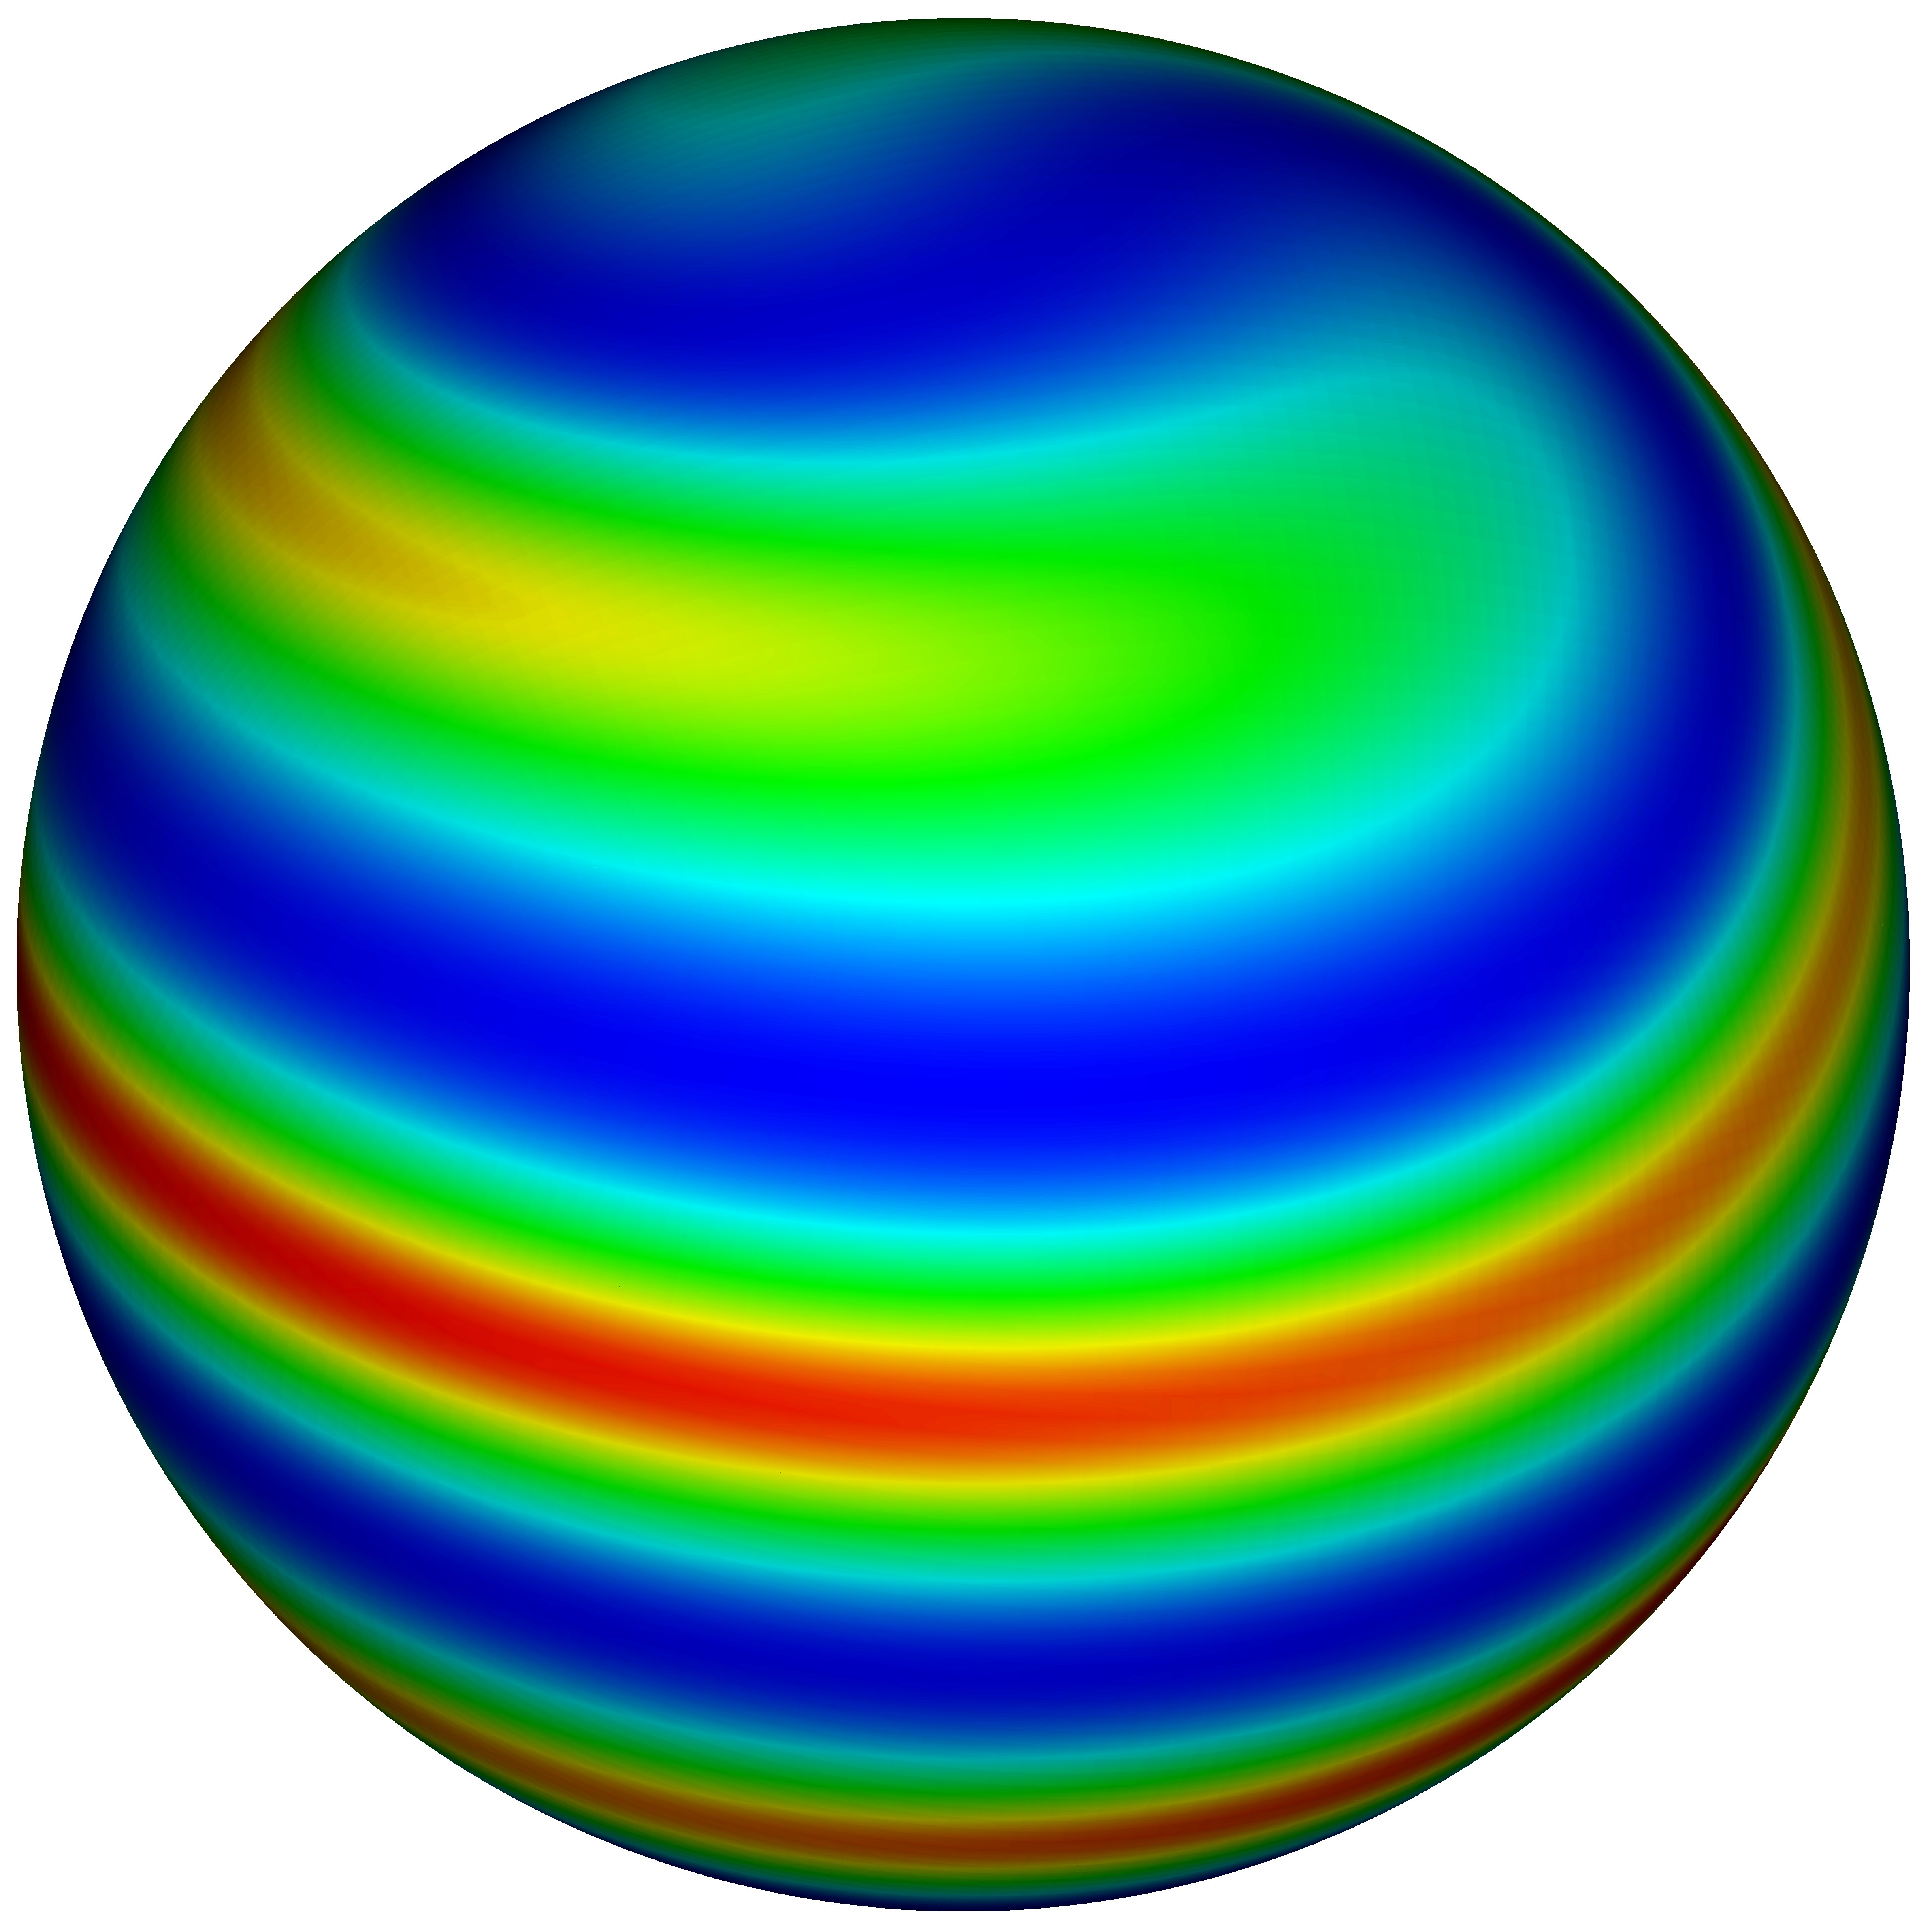
\includegraphics[height=6cm]{figures/front_simu.jpg} 
\end{center} 


\textbf{Résumé :} 
\vspace{0.3cm}

\textbf{Mots clefs :} cailloux, galet de référence
\vspace{0.3cm}


\end{titlepage}

\newpage

\renewcommand\thepage{}

\section*{Remerciements}




\tableofcontents


\newpage
\renewcommand\thepage{\arabic{page}}
\setcounter{page}{1}


\definecolor{linkcolor}{rgb}{0,0,1}

%%%%%%%%%%%%%%%%%%%%%%%%%%%%%%%%%%%%%%%%%%%%%%%%%%%%%%%%%%%%%%%%%%%%%%%%%%%%%%%%%%%%%%%%
%%%%%%%%%%%%%%%%%%%%%%%%%%%%%%%%%%%%%%%%%%%%%%%%%%%%%%%%%%%%%%%%%%%%%%%%%%%%%%%%%%%%%%%%
\section*{Introduction}
%%%%%%%%%%%%%%%%%%%%%%%%%%%%%%%%%%%%%%%%%%%%%%%%%%%%%%%%%%%%%%%%%%%%%%%%%%%%%%%%%%%%%%%%
%%%%%%%%%%%%%%%%%%%%%%%%%%%%%%%%%%%%%%%%%%%%%%%%%%%%%%%%%%%%%%%%%%%%%%%%%%%%%%%%%%%%%%%%
\addcontentsline{toc}{section}{Introduction}


\newpage
%%%%%%%%%%%%%%%%%%%%%%%%%%%%%%%%%%%%%%%%%%%%%%%%%%%%%%%%%%%%%%%%%%%%%%%%%%%%%%%%%%%%%%%%
%%%%%%%%%%%%%%%%%%%%%%%%%%%%%%%%%%%%%%%%%%%%%%%%%%%%%%%%%%%%%%%%%%%%%%%%%%%%%%%%%%%%%%%%
\section{Premiere partie}
%%%%%%%%%%%%%%%%%%%%%%%%%%%%%%%%%%%%%%%%%%%%%%%%%%%%%%%%%%%%%%%%%%%%%%%%%%%%%%%%%%%%%%%%
%%%%%%%%%%%%%%%%%%%%%%%%%%%%%%%%%%%%%%%%%%%%%%%%%%%%%%%%%%%%%%%%%%%%%%%%%%%%%%%%%%%%%%%%

\subsection{Première sous partie}



\section{Quelques formules}
Remarque : $\frac{\partial F}{\partial x}$ sera noté $\partial_x F$


Équation de la chaleur avec terme de production:

\begin{equation}
\rho C_p \partial_t T = div ( \lambda \vec{grad}(T))  + P
\end{equation}

À 1d ca devient 

\begin{equation}
\rho C_p \partial_t T = \partial_x ( \lambda \partial_x T)  + P
\end{equation}


 À 3D en symétrie sphérique ça devient :

\begin{equation}
\rho C_p \partial_{t'} T = \frac{1}{r'^2} \partial_{r'} ( \lambda {r'}^2 \partial_{r'} T)  + P
\end{equation}

En unités adimensionnées 3D en symétrie sphérique ça devient :
\begin{align}
r &= r'/R_{T} \\
t &= t' \frac{\lambda}{\rho C_p R_{T}^2} \\
p &= \frac{P R_{T}^2 }{ \lambda}\\
\partial_{t}T &= \frac{1}{r^2} \partial_{r} ({r}^2 \partial_{r} T)  + p
\end{align}




\subsection{discretisation}

On note $T(t,r_i) $ : $  T^t_i$
\begin{align}
\partial_t T &\rightarrow  \frac{T^{t+1}_r - T^{t+1}_r}{\Delta t}\\
\partial_r T &\rightarrow  \frac{T^t_{i+1/2} - T^{t}_{i-1/2}}{\Delta r} \\
\frac{1}{r^2}\partial_r (r^2 \partial_r T ) &\rightarrow \frac{1}{r^2_i \Delta r}\Big [ r^2_{i+1/2}\frac{T^t_{i+1} - T^{t}_{i}}{\Delta r} + r^2_{i-1/2}\frac{T^t_{i-1} - T^{t}_{i}}{\Delta r} \Big]
\end{align}

\subsection{équation implicite}

\begin{multline}
\frac{T^{t+1}_i - T^{t}_i}{\Delta t} = \frac{1}{r^2_i \Delta r}\Big [ r^2_{i+1/2}\frac{T^{t+1}_{i+1} - T^{t+1}_{i}}{\Delta r} + r^2_{i-1/2}\frac{T^{t+1}_{i-1} - T^{t+1}_{i}}{\Delta r} \Big] + p^t_i \\
T^{t+1}_i + \frac{\Delta t}{r^2_i \Delta r^2}\Big [ r^2_{i+1/2}(T^{t+1}_{i} - T^{t+1}_{i+1}) + r^2_{i-1/2}(T^{t+1}_{i}- T^{t+1}_{i-1}) \Big]  =
 T^{t}_r  + \Delta t ~ p^t_i
\end{multline}

On a ainsi l'équation matricielle implicite suivante : $ MT^{t+1} = T^t $


Où :
$
M = \Big [ Id + \frac{\Delta t ~ r^2_{i+1/2}}{r^2_i \Delta r^2} ~ d1 + \frac{\Delta t ~ r^2_{i-1/2}}{r^2_i \Delta r^2} ~ d2  \Big]
$

\begin{equation}
d1=
\begin{bmatrix}
    2      & -1     & -1        & 0     &\dots      & 0 \\
    0      &  1     & -1        & 0     &           & \vdots  \\
    \vdots & \ddots & \ddots    &\ddots & \ddots    & \vdots \\
    \vdots &        & \ddots    &\ddots & \ddots    & 0 \\
    \vdots &        &           &\ddots & 1         &  -1 \\
    0      & \dots  & \dots     &\dots  & 0         &  0
\end{bmatrix}
d2=
\begin{bmatrix}
     0     & 0      & \dots  & \dots    &\dots      & 0 \\
    -1     & 1      & \ddots &          &           & \vdots  \\
    0      & \ddots & \ddots & \ddots   &           & \vdots \\
    \vdots & \ddots & \ddots & \ddots   & \ddots    & \vdots \\
    \vdots &        & 0      &  -1      &  1        & 0\\
    0      & \dots  & 0      &  -1      & -1        & 2 \\
\end{bmatrix}
\end{equation}

$ \rho L \frac{\partial \phi}{\partial t} = \rho L \frac{d \phi}{d T}\frac{\partial T}{\partial t} $ avec $\phi$ qui est une marche, on peut l'approximer par une fonction un peu plus dérivable par ex :  $\phi \simeq arctan(T-T_{fusion})$ 

$ \rho Cp_{eff} = \rho Cp(\phi) + \rho L  \frac{d \phi}{d T}$



$R_T = a t^b , T = T(t,r/R_T(t)) $

$\Rightarrow \frac{\partial T(t,r/R_T(t))}{\partial t}  = \frac{\partial T}{\partial t} + \frac{\partial \frac{r}{R_T(t)}}{\partial t}\frac{\partial T}{\partial r} = \frac{\partial T}{\partial t} + \frac{\partial \frac{r}{R_T(t)}}{\partial t}\frac{\partial T}{\partial r} $

\section{Modèles}

Note pour tous les modèles suivants on supposera que la Terre est composée d'un mélange homogène de $\phi = $18\% de métal et 82\% de silicates. Et que les propriétés de ces matériaux ne changent pas avec la température ou le changement d'état.

Les constantes respectives et moyennes du mélange sont les suivantes :
\tabulinesep=0.3mm
\begin{center}
  \begin{tabu}{ r | c c c l}
    Grandeur & moyenne & metal & silicate & unité\\ \hline
    Densité ($\rho$) & 4028 & 7800 &  3200 & \SI{}{kg.m^{-3}}\\ \hline
    Capacité calorifique ($C_p$) & 1065 & 450 & 1200 &  \SI{}{J.K^{-1}.kg^{-1}} \\ \hline
    Conductivité & 11.48 & 50 & 3 & \SI{}{W.K^{-1}.m^{-1}}  \\ \hline    
    Chaleur latente de fusion & & 250 & 500 & \SI{}{kJ.kg^{-1}}\\ \hline
    Température de fusion & & 1261 & 1408 & \SI{}{K}\\ \hline

  \end{tabu}
\end{center}

Pour la suite $\rho$ désignera une valeur moyenne et $\rho_{materiau}$ la valeur respective d'un des matériaux.


\subsection{Modèle 1}

Fichier : sim1.py

\subsubsection{Description}

On fait une première simulation la plus simple possible.
Hypothèses : 
\begin{enumerate}
\item Rayon de la Terre constant 
\item Chauffage causé par la désintégration du $^{26}$Al et par le rayonnement de corps noir.
\end{enumerate}

\subsubsection{Données initiales et constantes}

\begin{center}
  \begin{tabu}{ r  c }
    \hline
    Rayon de la Terre & \SI{500}{km} \\ \hline
    Température initiale & \SI{300}{K}  \\ \hline
    Température de la nébuleuse & \SI{300}{K}  \\ \hline
    Demi-vie du $^{26}$Al & \SI{0.74}{My}  \\ \hline
  \end{tabu}
\end{center}

\subsubsection{Équations}

On considère les variables adimentionnées suivantes: 


\begin{equation}
t= \frac{t'}{\tau^{Al}_{1/2}}  \quad \textrm{,} \quad   r = r' \sqrt{\frac{\rho C_p} {k_T \tau_{1/2}}} \quad  \textrm{et} \quad T = \frac{T'}{T_0} 
\end{equation}

Il en résulte l'équation suivante :


\begin{equation}
\frac{\rho C_p T_0}{\tau_{1/2}} \partial_{t} T = \frac{\rho C_p T_0}{\tau_{1/2}} \frac{1}{r^2} \partial_{r} ( {r}^2 \partial_{r} T)  + P + S ~(+ ~Q_L)
\end{equation}


Avec :
\begin{equation}
 P = \rho H_0 e^{-ln(2) t} 
\end{equation}

%Pour passer d'une puissance surfacique à une puissance volumique on introduit 1/delta r
\begin{equation}
 S =\frac{\sigma}{\Delta r}(T_{neb}^4 - (TT_0)^4)  \quad \textrm{à la surface uniquement}
\end{equation}

$Q_L$ représente la chaleur "perdue" lors du changement de phase de chaque matériau. Ce changement de phase est géré en dehors de l'équation de la chaleur. On note $\phi_{met}$ la proportion solide/liquide du métal et $\phi_{sil}$ pour le silicate ($\phi_{sil} = 0 \Rightarrow$ solide, $\phi_{sil} = 1 \Rightarrow$ liquide). On detecte le changement de phase solide $\rightarrow$ liquide du métal par la condition  $T > T_{fus,met} $ et $ \phi_{met} < 1$ on "échange" alors de la température contre du changement de phase de sorte à obtenir soit $T = T_{fus,met}$ soit $\phi_{met} = 1$. On fait de même avec la transition inverse et avec le silicate.

Exemples : on part de $T > T_{fus,met}$ , $ \phi_{met} < 1$ 


Cas 1 on atteint $\phi_{met} = 1$. Calculons la température finale : 

\begin{equation}
T_{f} =  T_{i} +  (\phi_{met} - 1 ) \frac{\phi L_{met}}{C_{p,met} }
\end{equation}

Cas 2 on atteint $T = T_{fus,met}$. Calculons le $\phi_{met}$ final : 

\begin{equation}
\phi_{f} =  \phi_{i} +  (T_{i}-T_{fus,met}) \frac{C_{p,met}}{\phi L_{met}}
\end{equation}

\subsubsection{Équations discrétisées}

On pose $c_0 = \frac{\tau_{1/2}}{\rho C_p T_0}$ 

On a l'équation matricielle suivante :
\begin{equation}
MT^{t+1} = T^t + c_0 \Delta t( P + S )
\end{equation}

Avec la matrice $M$ calculée plus tôt : 
$
M = \Big [ Id + \frac{\Delta t ~ r^2_{i+1/2}}{r^2_i \Delta r^2} ~ d1 + \frac{\Delta t ~ r^2_{i-1/2}}{r^2_i \Delta r^2} ~ d2  \Big]
$

\begin{equation}
d1=
\begin{bmatrix}
    2      & -1     & -1        & 0     &\dots      & 0 \\
    0      &  1     & -1        & 0     &           & \vdots  \\
    \vdots & \ddots & \ddots    &\ddots & \ddots    & \vdots \\
    \vdots &        & \ddots    &\ddots & \ddots    & 0 \\
    \vdots &        &           &\ddots & 1         &  -1 \\
    0      & \dots  & \dots     &\dots  & 0         &  0
\end{bmatrix}
d2=
\begin{bmatrix}
     0     & 0      & \dots  & \dots    &\dots      & 0 \\
    -1     & 1      & \ddots &          &           & \vdots  \\
    0      & \ddots & \ddots & \ddots   &           & \vdots \\
    \vdots & \ddots & \ddots & \ddots   & \ddots    & \vdots \\
    \vdots &        & 0      &  -1      &  1        & 0\\
    0      & \dots  & 0      &  -1      & -1        & 2 \\
\end{bmatrix}
\end{equation}

%%%%%%%%%%%%%%%%%%%%%%%%%%%%%%%%%%%%%%%%%%%%%%%%%%%%%%%%%%%%%%%%%%%%%%%%%%%%%%%%%%%%%%%%
%%%%%%%%%%%%%%%%%%%%%%%%%%%%%%%%%%%%%%%%%%%%%%%%%%%%%%%%%%%%%%%%%%%%%%%%%%%%%%%%%%%%%%%%
\section*{Conclusion}
%%%%%%%%%%%%%%%%%%%%%%%%%%%%%%%%%%%%%%%%%%%%%%%%%%%%%%%%%%%%%%%%%%%%%%%%%%%%%%%%%%%%%%%%
%%%%%%%%%%%%%%%%%%%%%%%%%%%%%%%%%%%%%%%%%%%%%%%%%%%%%%%%%%%%%%%%%%%%%%%%%%%%%%%%%%%%%%%%
\addcontentsline{toc}{section}{Conclusion}


\newpage
%%%%%%%%%%%%%%%%%%%%%%%%%%%%%%%%%%%%%%%%%%%%%%%%%%%%%%%%%%%%%%%%%%%%%%%%%%%%%%%%%%%%%%%
%%%%%%%%%%%%%%%%%%%%%%%%%%%%%%%%%%%%%%%%%%%%%%%%%%%%%%%%%%%%%%%%%%%%%%%%%%%%%%%%%%%%%%%
\appendix
%%%%%%%%%%%%%%%%%%%%%%%%%%%%%%%%%%%%%%%%%%%%%%%%%%%%%%%%%%%%%%%%%%%%%%%%%%%%%%%%%%%%%%%
%%%%%%%%%%%%%%%%%%%%%%%%%%%%%%%%%%%%%%%%%%%%%%%%%%%%%%%%%%%%%%%%%%%%%%%%%%%%%%%%%%%%%%%
\section{Première annexe} \label{annexe_fonctionnelles}


\newpage
\bibliographystyle{unsrt}
\bibliography{rapport} 
\addcontentsline{toc}{section}{Références} 


\end{document}
